\section{Zielsetzung}
Ziel des Versuches ist es, mit Hilfe der Debye-Scherrer Methode, Eigenschaften
über Strukturen von Metallen und Salzen zu ermitteln. Innerhalb dieses
Versuches wird mittels der Debye-Scherrer Aufnamen Rückschlüsse über die
Netzebenabstände und die Struktur der Elementarzellen geschlossen.


\section{Theorie}
\label{sec:Theorie}
Die zu untersuchende Materie weißt kristalline Strukturen auf, sodass zuerst
innerhalb der Theorie auf die verschiedenen Kristallstrukturen eingegangen wird.\\
\subsection{Grundlagen zur Kristallstrukturen}
Kristalle bestehen aus einer periodisch angeordneten Basis, welche für
verschiedene Kristalle aus einem oder mehreren Atomen bestehen kann.
Die Form und die periodische Anordnung im Raum legen fest,
was für eine Kristallstruktur vorliegt. \\
Durch die Tranlation im Raum entsteht ein Gitter aus Basisvektoren, welches
eine Linearkombination $\vec l$ der möglichen fundamentalen Translationen in
jede Richtung des Raums ist
$$ \vec l = n_1 \vec a + n_2 \vec b + n_3 \vec c .$$
Die Faktoren $n_1-n_3 $
Abbildung
\begin{figure}
    \centering
    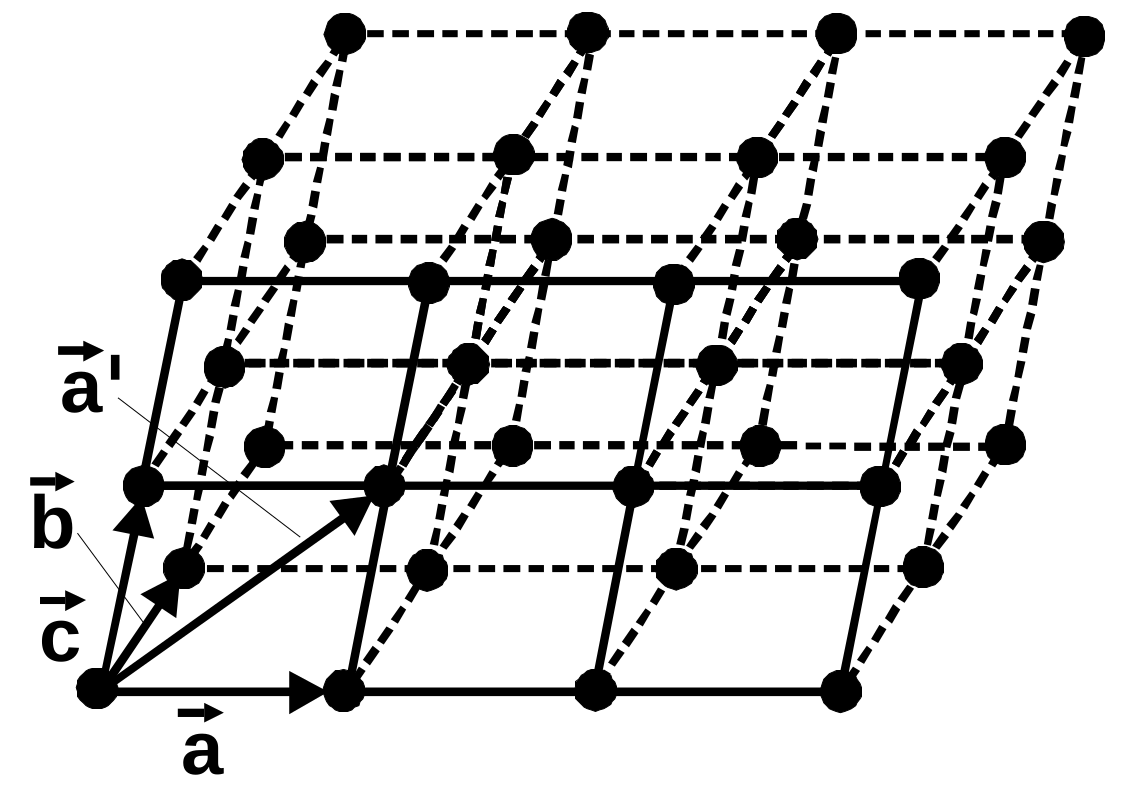
\includegraphics[width=0.55\textwidth]{ressources/gitter.png}
    \caption{Eines Gitters mit verschiedenen Gitterpunkten und deren mögliche
    Verschiebung durch den Translationsvektor $\vec l$.}
    \label{fig_gitter}
\end{figure}
\ref{fig_gitter}
 stellt eine mögliche Anordnung eines Gitters mit
einer einatomigen Basis dar (Punktgitter). Jeder Punkt des Gitters kann von
jedem Punkt durch die Linearkombination $\vec l$ erreicht werden.
\subsection{Elementarzelle}
Eine Elementarzelle definiert die kleinste Einheit einer Kristallstruktur.
Es wird zwischen primitive Einheitszellen und Einheitszellen mit mehreren Atomen
(z.B. Salze) unterschieden. Im Fall einer primitiven Einheitszelle
liegt auf jeder Ecke der Einheitszelle das selbe Atome. Das heißt die Gitterpunkte
bilden gleichzeitig auch das Kristallgitter. In der Abbildung \ref{primitiv} ist
eine kubisch primitive Einheitszelle dargestellt, einer der Eckpunkte kann
als primitive Einheitszelle festgelegt werden.

\begin{figure}
    \centering
    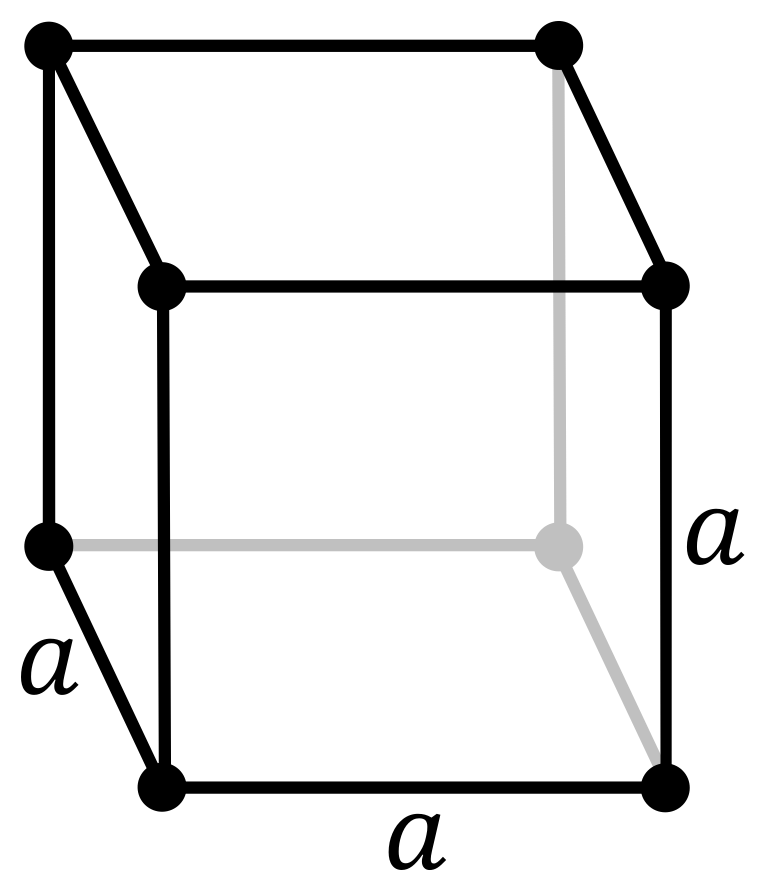
\includegraphics[width=0.25\textwidth]{ressources/primitiv.png}
    \caption{Eines Gitters mit verschiedenen Gitterpunkten und deren mögliche
    Verschiebung durch den Translationsvektor $\vec l$.}
    \label{primitiv}
\end{figure}


Bei Einheitszellen
mit mehreren Atomen wie z.B. NaCl besteht die Einheitszelle aus $\text{Na}^+$
und $\text{Cl}^-$ Ionen.
% 2x2 Plot
% \begin{figure*}
%     \centering
%     \begin{subfigure}[b]{0.475\textwidth}
%         \centering
%         \includegraphics[width=\textwidth]{Abbildungen/Schaltung1.pdf}
%         \caption[]%
%         {{\small Schaltung 1.}}
%         \label{fig:Schaltung1}
%     \end{subfigure}
%     \hfill
%     \begin{subfigure}[b]{0.475\textwidth}
%         \centering
%         \includegraphics[width=\textwidth]{Abbildungen/Schaltung2.pdf}
%         \caption[]%
%         {{\small Schaltung 2.}}
%         \label{fig:Schaltung2}
%     \end{subfigure}
%     \vskip\baselineskip
%     \begin{subfigure}[b]{0.475\textwidth}
%         \centering
%         \includegraphics[width=\textwidth]{Abbildungen/Schaltung4.pdf}    % Zahlen vertauscht ... -.-
%         \caption[]%
%         {{\small Schaltung 3.}}
%         \label{fig:Schaltung3}
%     \end{subfigure}
%     \quad
%     \begin{subfigure}[b]{0.475\textwidth}
%         \centering
%         \includegraphics[width=\textwidth]{Abbildungen/Schaltung3.pdf}
%         \caption[]%
%         {{\small Schaltung 4.}}
%         \label{fig:Schaltung4}
%     \end{subfigure}
%     \caption[]
%     {Ersatzschaltbilder der verschiedenen Teilaufgaben.}
%     \label{fig:Schaltungen}
% \end{figure*}
